% План на главу
% 0) Фотонное излучение от радионуклидов
% 1) Описать про датчики в системе аскро и их характеристики (дальность, макс мощность и тд)
% 2) Описать, зачем в модели аскро нужны датчики
% 3) Описать формулу для расчета
% 4) Описать реализацию непосредственно в коде
% ПРОВЕРИТЬ НА ОРФОГРАФИЮ!!

\chapter{Разработка модуля расчета мощности дозы внешнего гамма-излучения}
\label{chapter_dose}

\section{Необходимость расчета мощности дозы гамма-излучения}

Радиоактивные нуклиды, которые могут попасть в атмосферу в результате аварии на \ac{aes}, являются бета-активными. При 
протекании бета-распада результирующее ядро может оказаться в возбужденном состоянии. Возбуждение ядра снимается 
посредством испускания гамма-квантов. Для примера, на рисунке \ref{fig_I_133_decay_gamma} представлена упрощенная схема 
распада изотопа $^{131}I$, после которого образуется изотоп $^{131}Xe$ в возбужденном состоянии, испускающий 
гамма-кванты при переходе в основное состояние.

\begin{figure}[ht!]
    \centering
    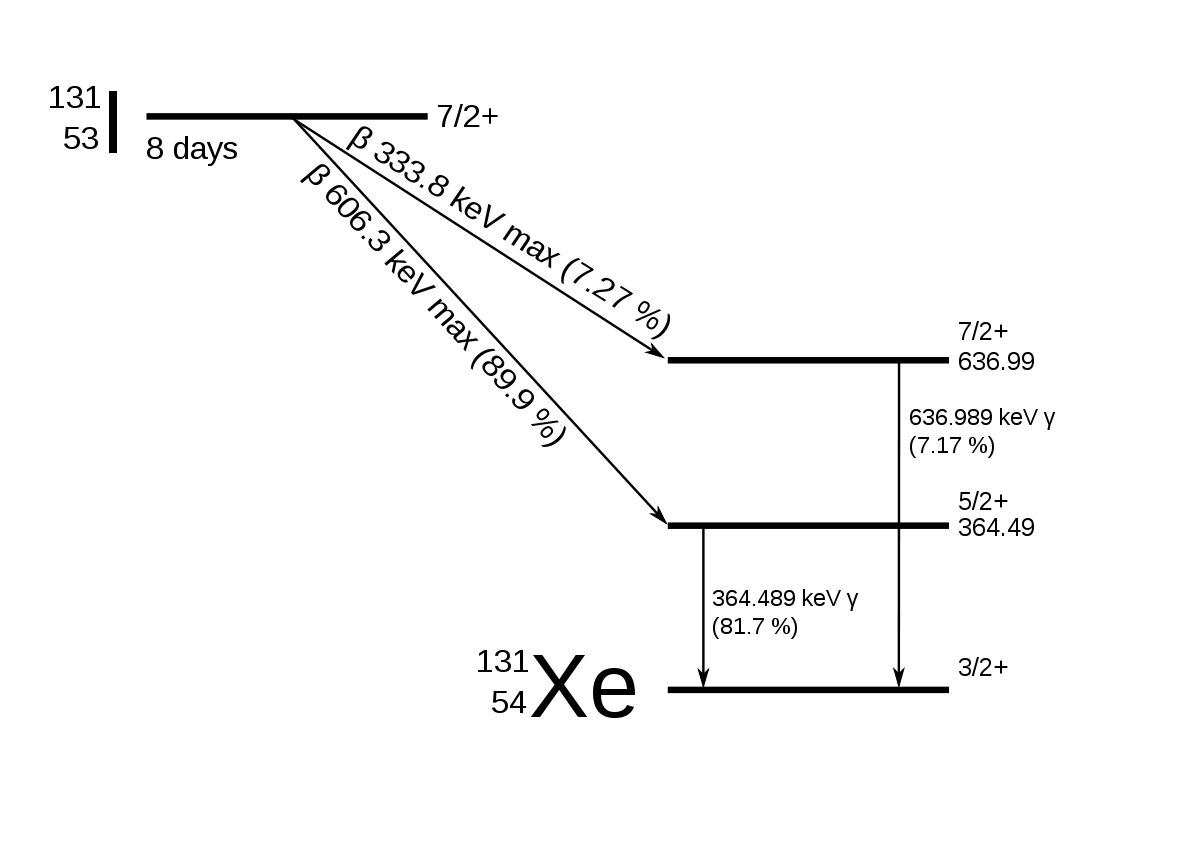
\includegraphics[width=13cm]{I_133_decay_gamma}
    \captionsetup{justification=centering}
    \caption{Упрощенная схема распада изотопа $^{131}I$.}
    \label{fig_I_133_decay_gamma}
\end{figure}

Одной из главных задач современных систем \ac{ascro} на \ac{aes} является измерение значений мощности дозы 
гамма-излучения на прилегающей к \ac{aes} местности. Значение мощности дозы гамма-излучения на местности необходимо знать 
для контроля радиационной обстановки вокруг \ac{aes}, а также своевременной выдаче рекомендаций по принятию решений о 
защите населения. Измерение мощности дозы гамма-излучения в системах \ac{ascro} проводится при помощи 
специализированных датчиков радиационного контроля, расположенных на прилегающей к \ac{aes} местности. 

\section{Датчики радиационного контроля}

Основу \ac{ascro} составляет система постов радиационного контроля гамма-излучения, расположенных вокруг \ac{aes}. 
Обычно, измерительные блоки фотонного излучения содержат датчики двух диапазонов: $10^-7$ - $10^-3$ Зв и $10^-3$ - $10$ 
Зв. В качестве блоков детектирования в системах постов радиационного контроля \ac{ascro} используются БДМГ-08Р3, БДМГ-08Р4, 
БДМГ-08Р5, БДМГ-100 \cite{elokhin}. Для примера, рассмотрим технические характеристики блока детектирования БДМГ-100.

Блок детектирования БДМГ-100 предназначен для непрерывного измерения мощности амбиентного эквивалента дозы 
гамма-излучения \cite{bdmg-100}. Блок применяется для контроля радиационной обстановки на объектах атомной энергетики 
и радиохимического производства; на промышленных предприятиях, использующих источники ионизирующих излучений; 
на пунктах специального и таможенного контроля и в службах экологического и санитарно-эпидемиологического надзора. В 
таблице ... приведены основные техническите характеристики блока детектирования БДМГ-100.

Измерение мощности дозы гамма-излучения в системах \ac{ascro} выполняется при помощи датчиков радиационного контроля, 
размещенных вокруг \ac{aes}. Одной из важнейших задач проектирования систем \ac{ascro} является их оптимизация. Под 
оптимизацией \ac{ascro} понимается выбор необходимого и достаточного количества датчиков радиационного контроля, 
размещенных вокруг \ac{aes}, а также методы их размещения, при помощи которых можно повысить точность прогностических 
расчетов при оценке уровней радиационного загрязнения подстилающей поверхности, дозовых нагрузок на персонал и население 
в случае радиационной аварии.
